\documentclass{homework}
\usepackage{lipsum}
\usepackage{cancel}
\usepackage{amsthm}
\usepackage{cleveref}
\usepackage{upgreek}
\usepackage{mathrsfs}
\usepackage{tikz}
\usepackage{units}
\usepackage{slashbox}
\newtheorem{lemma}{Lemma}

\DeclareMathOperator{\cov}{cov}

\title{Kevin Joyce}
\course{Stat 542 - Applied Linear Models - Homework 5}
\author{Kevin Joyce}
\docdate{\today}
\begin{document} 
\newcommand{\figref}[1]{\figurename~\ref{#1}}
\renewcommand{\bar}{\overline}
\renewcommand{\hat}{\widehat}
\renewcommand{\SS}{\mathcal S}
\newcommand{\HH}{\mathscr H}
\newcommand{\mom}{\widetilde}
\newcommand{\mle}{\widehat \Uptheta}
\newcommand{\eps}{\varepsilon}
\newcommand{\todist}{\stackrel{D}\longrightarrow}
\newcommand{\toprob}{\stackrel{p}\longrightarrow}
\newcommand{\TTheta}{\overline{\underline \Theta} }
\newcommand{\del}{\partial}
\newcommand{\approxsim}{\overset{\cdotp}{\underset{\cdotp}{\sim}}}
\newcommand{\RSS}{\ensuremath{\mathrm{RSS}}}
\newcommand{\MSE}{\ensuremath{\mathrm{MSE}}}
\newcommand{\SE}{\ensuremath{\mathrm{SE}}}
\newcommand{\TSS}{\ensuremath{\mathrm{TSS}}}
\newcommand{\SSReg}{\ensuremath{\mathrm{SSReg}}}
\renewcommand{\a}[1]{{\color{red} \it #1}}

\begin{longproblem}
Faraway 6.1. Researchers at the National Institutes of Standards and Technology (NIST) collected \texttt{pipeline} data on ultrasonic measurements of the depths of defects in the Alaska pipeline in the field.  The depth of the defects were then remeasured in the laboratory. These measurements were perfomred in six different batches.  It turns out that this batch effect is not significant and so can be ignored in the analysis that follows.  The laboratory measurements are more accurate than the in-field measurements, but more time consuming and expensive.  We want to develop a regression equation for the in-field measurements.  

\subproblem{ Fit a regression model \texttt{Lab \textasciitilde~Field}.  Check for nonconstant variance.}

\begin{minipage}{.5\textwidth}
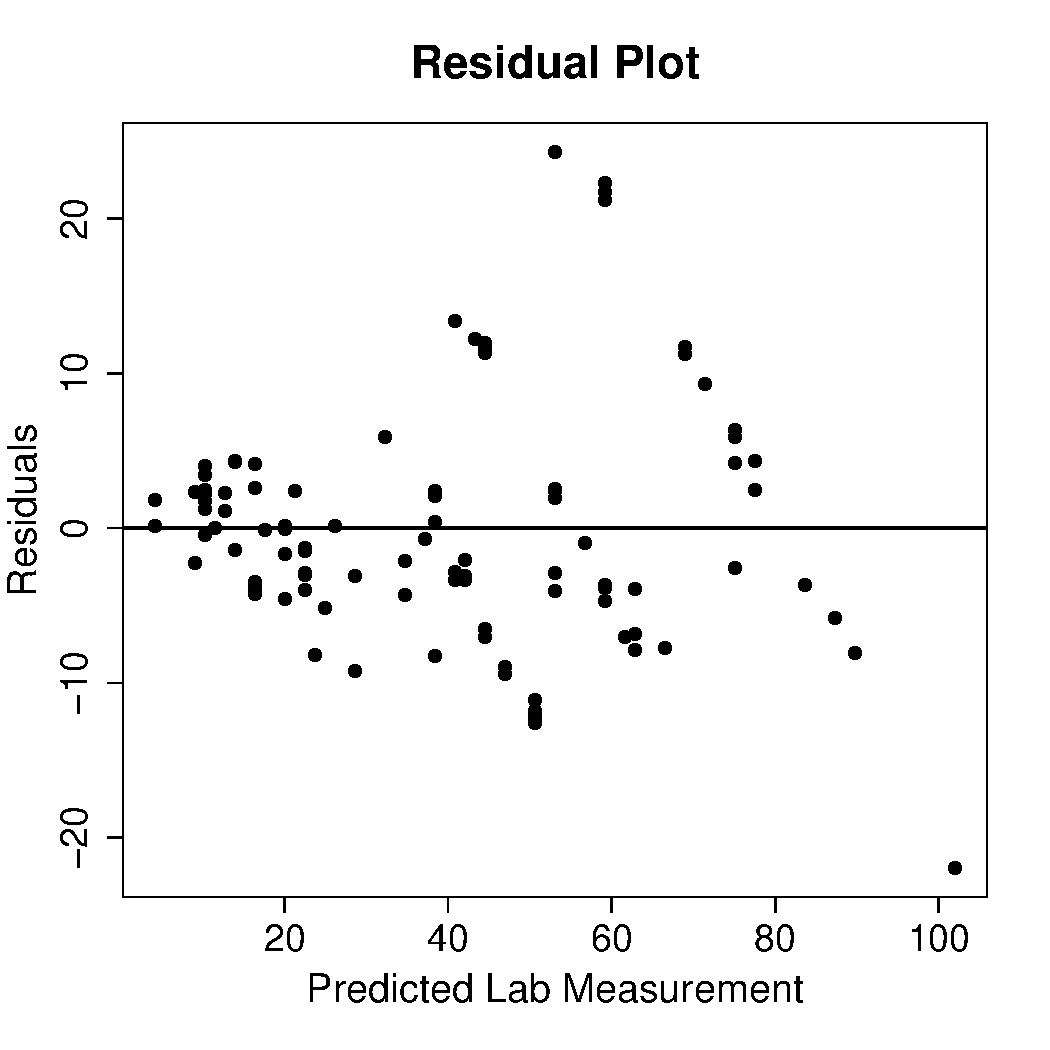
\includegraphics[width=\textwidth]{nist_resid.pdf}
\end{minipage}
\begin{minipage}{.5\textwidth}
Based on the residual plot to the left, there appears to be non-constant
variance.  That is, as the predicted lab measurement increases to 60, the
magnitude of the residuals increases. This indicates evidence for higher variance at those values.\end{minipage}

\begin{longsubproblem}We wish to use weights to account for the nonconstant variance. Here we split the range of \texttt{Field} into 12 groups of size nine (except for the last group which has only eight values).  Within each group, we compute the variance of \texttt{Lab} as \texttt{varlab} and the mean of \texttt{Field} as \texttt{meanfield}.  Assuming that the \texttt{pipeline} data has been attached, the following \texttt{R} code computes the group means and variances:
\begin{verbatim}
> sort_idx = order(Field) 
> grps = factor(ceiling(sort_idx/9))  # this factors into groups of size at most 9
> meanfield = tapply(Field,grps,mean)
> varlab = tapply(Lab,grps,var)
\end{verbatim}
Suppose we guess that the variance in the response is linked to the predictor in the following way:
$$
  var(Lab) = a_0Field^{a_1}.
$$
Regress \texttt{log(varlab)} on \texttt{log(meanfield)} to estimate $a_0$ and $a_1$.  (You might want to remove the last point.) Use this to determine appropriate weights in a WLS fit of \texttt{Lab} on \texttt{Field}.  Show the regression summary.
\end{longsubproblem}

\begin{solution}
Note that we must back transform the weights to follow the model above.  The following codes accomplish this.

\begin{minipage}{.5\textwidth}
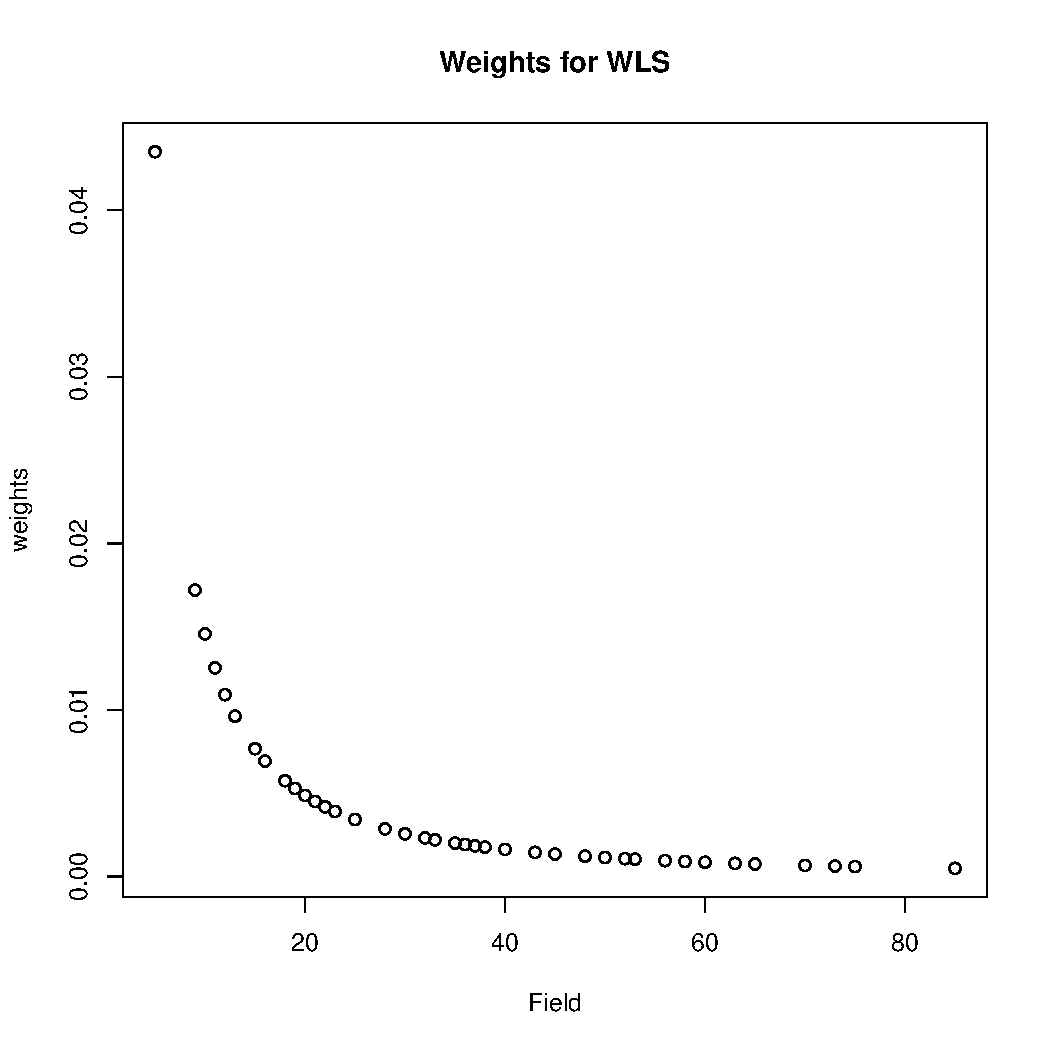
\includegraphics[width=.8\textwidth]{weights.pdf}
\end{minipage}
\begin{minipage}{.5\textwidth}
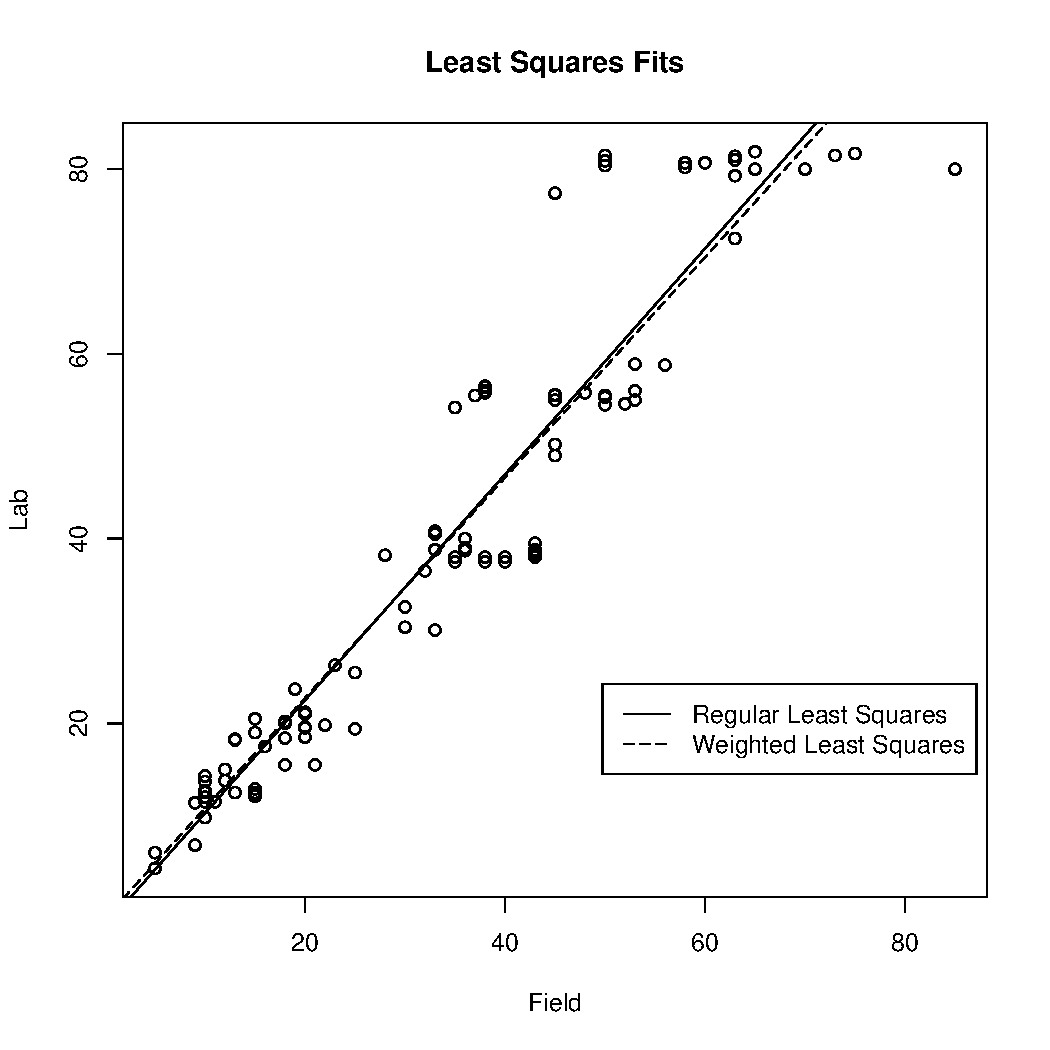
\includegraphics[width=.8\textwidth]{wls_nist.pdf}
\end{minipage}
\begin{minipage}{.5\textwidth}
{\small
\begin{verbatim}
> reg1 = lm(Lab ~ Field)
> reg2 = lm(Lab~Field,weight=weights) 
> wls_reg = lm(log(varlab)~log(meanfield))
> X = cbind(1,log(Field))
> weights = 1 / exp( X%*%coef(wls_reg) )
> reg2 = lm(Lab~Field,weight=weights)
> summary(reg2) 
Coefficients:
            Estimate Std. Error t value Pr(>|t|)    
(Intercept) -1.12747    0.72823  -1.548    0.125    
Field        1.19305    0.03407  35.018   <2e-16 ***
> summary(reg1)
Coefficients:
            Estimate Std. Error t value Pr(>|t|)    
(Intercept) -1.96750    1.57479  -1.249    0.214    
Field        1.22297    0.04107  29.778   <2e-16 ***
\end{verbatim}
}
\end{minipage}
\begin{minipage}{.5\textwidth}
\vspace{-2cm}
Note that according to our weighting scheme, the lowest \texttt{Field} value
has a very large weight on the model.  Observe the effect of the weighting on the
estimates of the coefficients is minor, but does give less influence to the  high variable points
near \texttt{Field} $\approx 60$.  Note also that the standard error for the slope has increased.
\end{minipage}
\end{solution}

\subproblem{ An alternative to weighting is transformation.  Find
transformations on \texttt{Lab} and/or \texttt{Field} so that in the
transformed scale the relationship is approximately linear with constant
variance.  You may restrict your choice of transformations to square root, log
and inverse.}

\vspace{-2em}
\begin{minipage}{.5\textwidth}
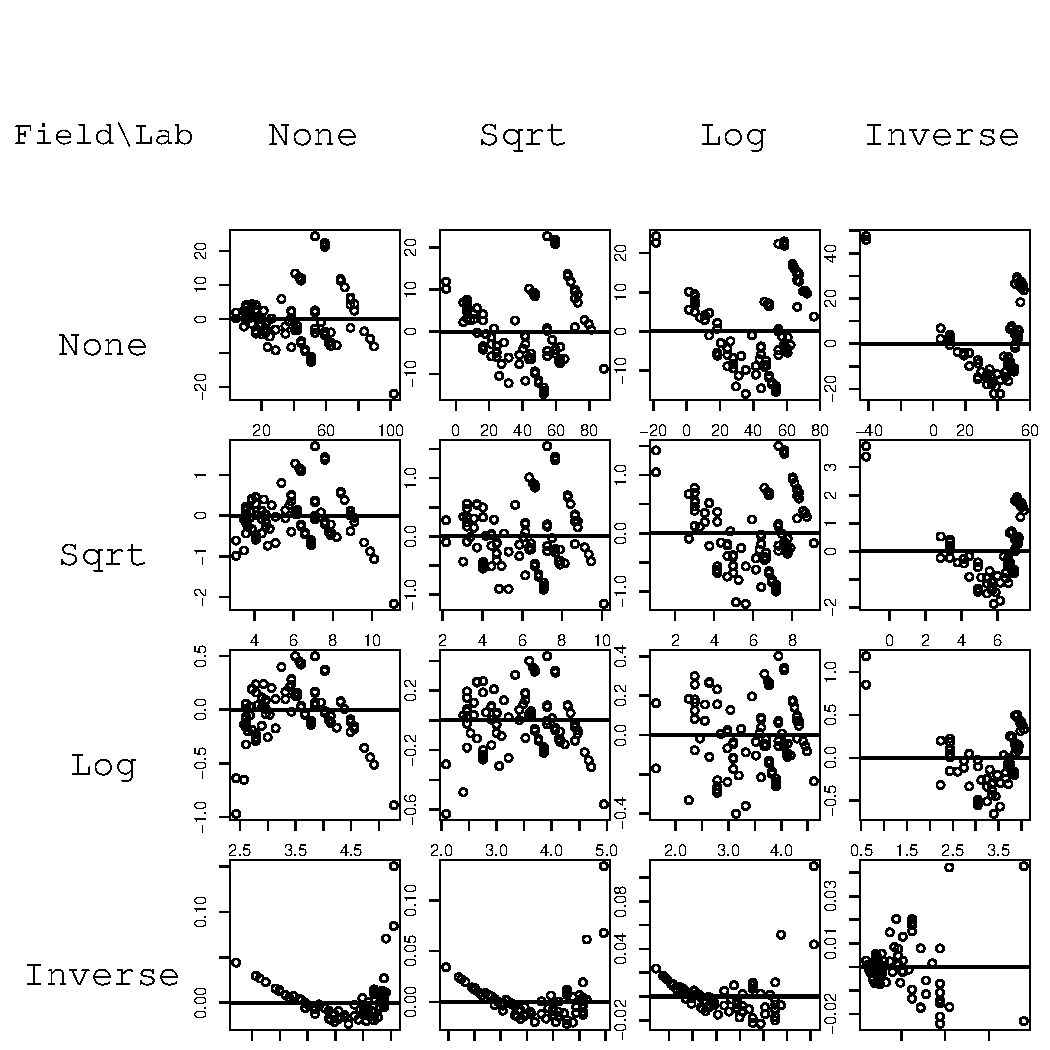
\includegraphics[width=\textwidth]{resid_matrix.pdf}
\end{minipage}
\begin{minipage}{.5\textwidth}
In this figure we plot the residual plots for the 16 possible transformation
combinations. The transformation is applied to \texttt{Lab} in each fixed
column and \texttt{Field} in each fixed row.  It is clear that the inverse
transformation is clearly not the thing to do in either the independent or
dependent variable.  Combinations of square root and log on both variables seem 
do better at reigning in heterogeneity, 
and the plot that appears to have the most homogeneity of
noise is log transformations on both \texttt{Lab} and \texttt{Field}.
\end{minipage}
\end{longproblem}

\begin{longproblem}
  Faraway 6.2. Using the \texttt{divusa} data, fit a regression model with
  \texttt{divorce} as the response and \texttt{unemployed, femlab, marriage,
  birth,} and \texttt{military} as predictors. 

  \subproblem{Make two graphical checks for correlated errors. What do you conclude? }
  \begin{solution}
\enlargethispage{2em}
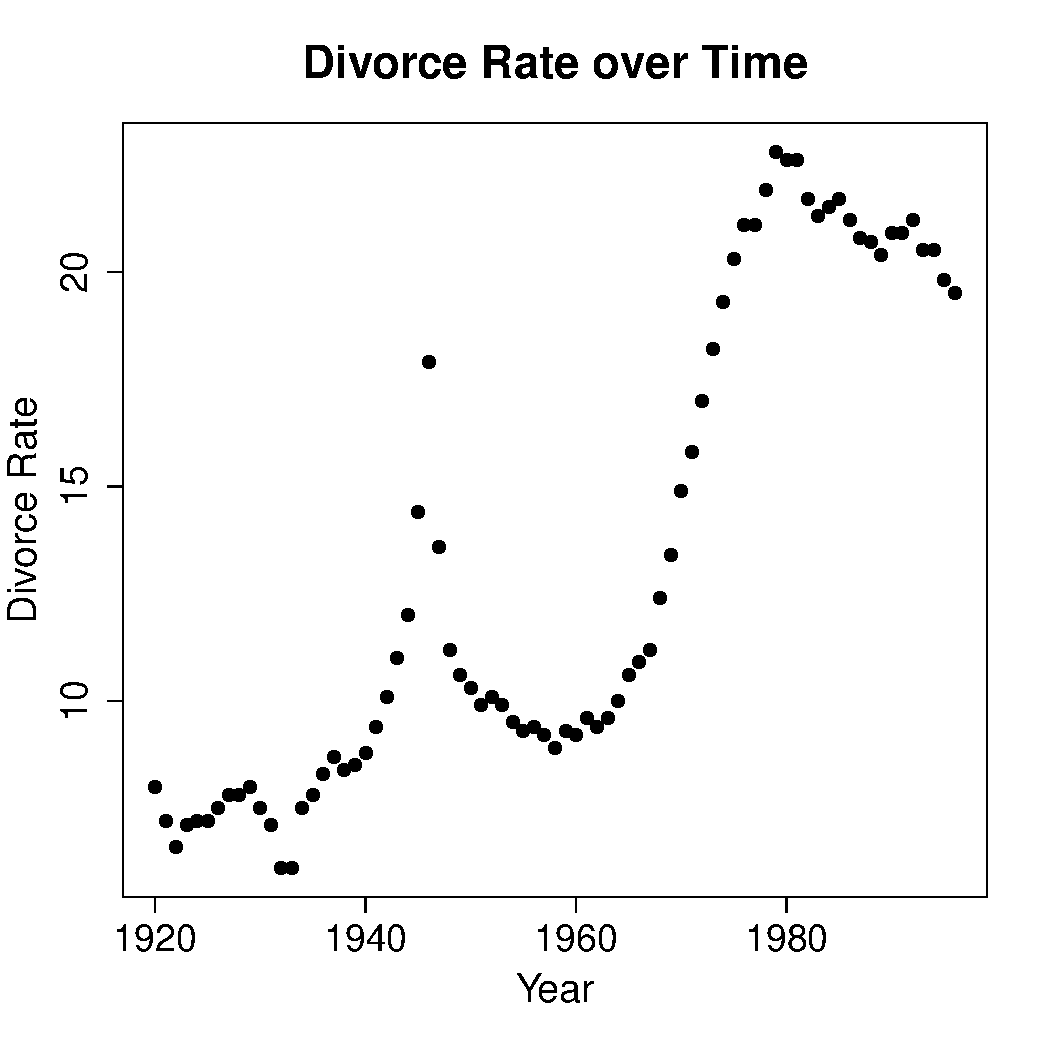
\includegraphics[width=.3\textwidth]{div_time.pdf}
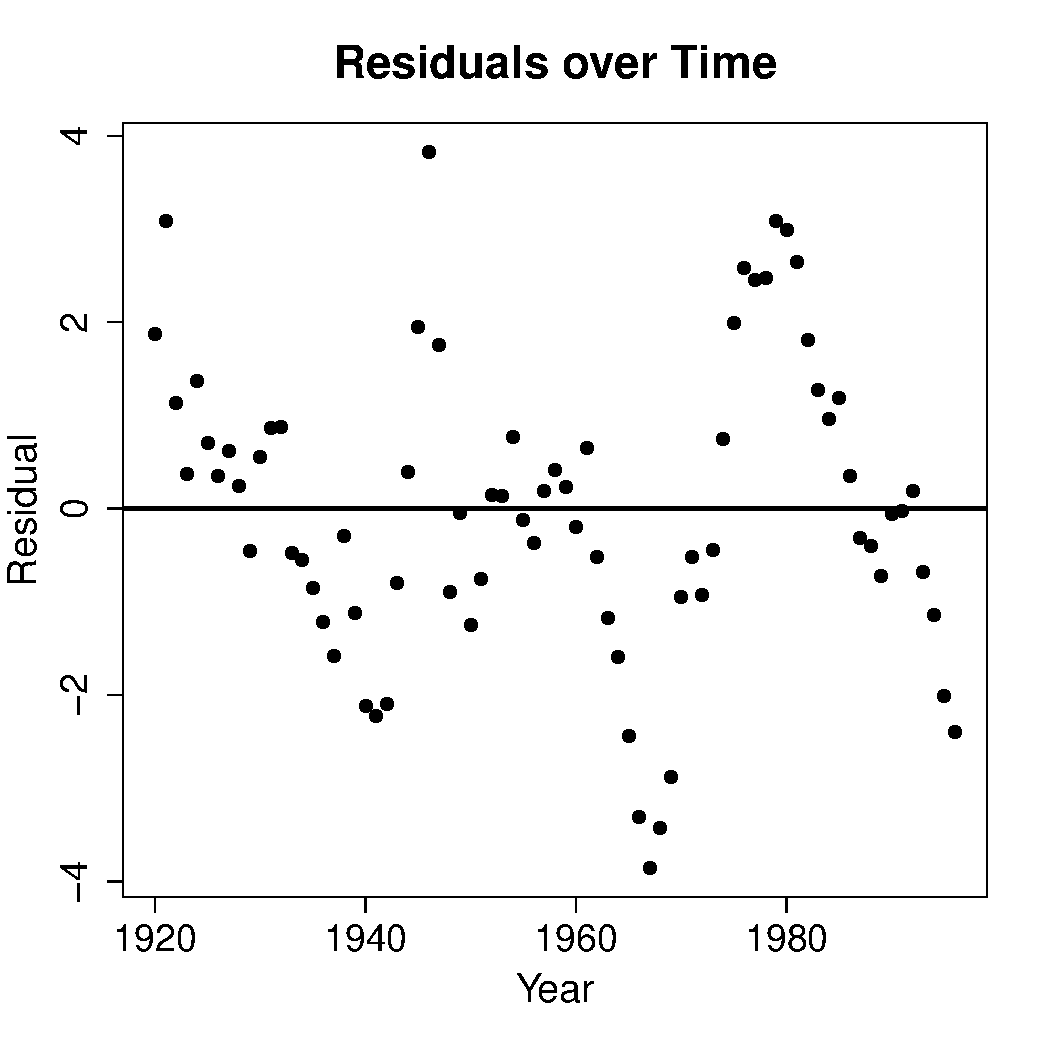
\includegraphics[width=.3\textwidth]{div_resid.pdf}
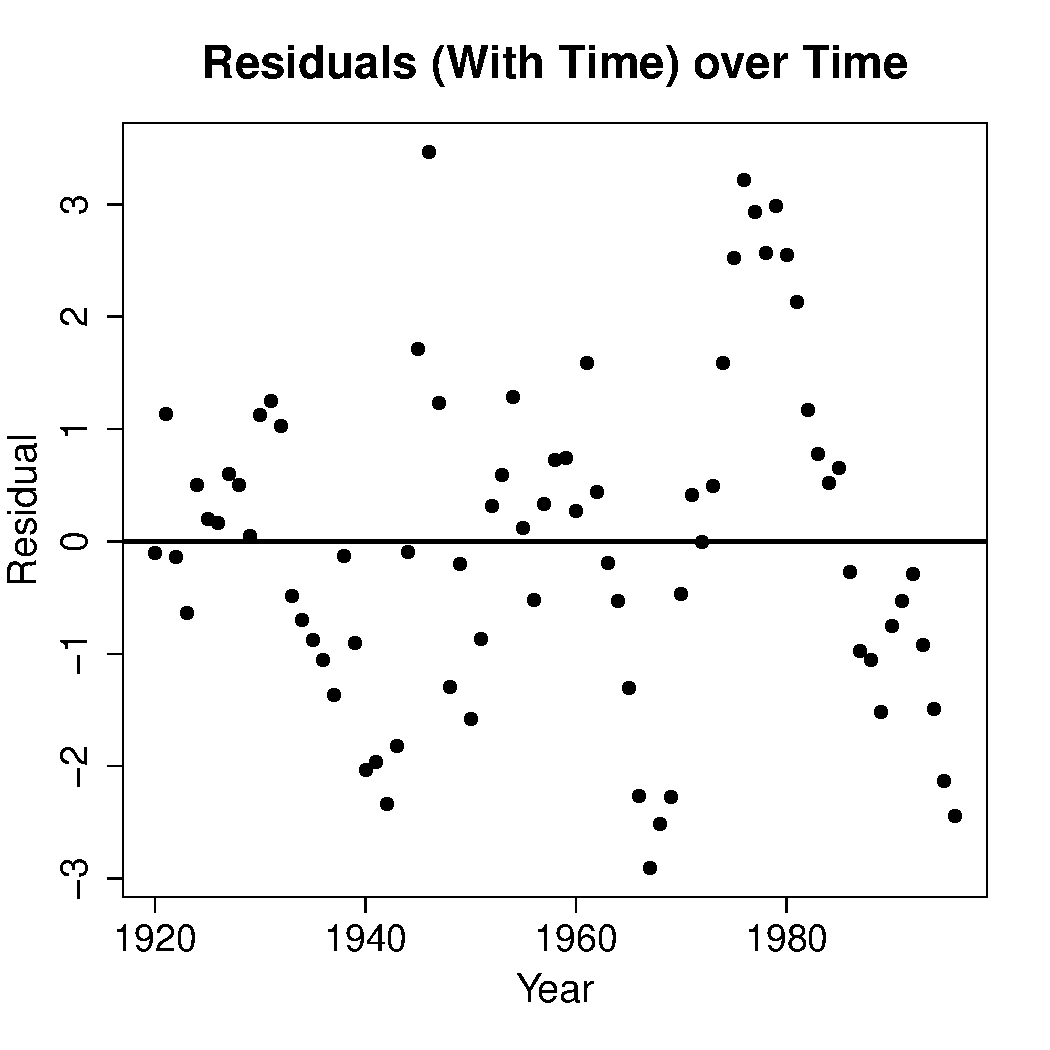
\includegraphics[width=.3\textwidth]{div_resid2.pdf}
As addressed in a previous homework (homework 4.2), there is a clear
correlation between the divorce rate and year as seen in the time plot to the
left. Fitting a least squares model and plotting the residuals versus time
indicates a lack independence in the estimates by the ``running'' pattern.
Adding \texttt{year} into the model does not resolve this issue (see the third
plot).
\end{solution}

  \subproblem{Allow for serial correlation with an AR(1) model for the errors.
  (Hint: Use maximum likelihood to estimate the parameters in the GLS fit by
  \texttt{gls(...,method="ML",...)} ).  What is the estimated correlation and
  is it significant?  Does the GLS model change which variables are found to be
  significant? }
\begin{minipage}{.5\textwidth}
\vspace{-3em}
{\footnotesize
\begin{verbatim}
Regular Least Squares Coefficients:
            Estimate Std. Error t value Pr(>|t|)    
(Intercept)  2.48784    3.39378   0.733   0.4659    
unemployed  -0.11125    0.05592  -1.989   0.0505 .  
femlab       0.38365    0.03059  12.543  < 2e-16 ***
marriage     0.11867    0.02441   4.861 6.77e-06 ***
birth       -0.12996    0.01560  -8.333 4.03e-12 ***
military    -0.02673    0.01425  -1.876   0.0647 .  
\end{verbatim}
}
\end{minipage}
\begin{minipage}{.5\textwidth}
{\footnotesize
\begin{verbatim}
Generalized Least Squares Coefficients:
                Value Std.Error   t-value p-value
(Intercept) -7.059682  5.547193 -1.272658  0.2073
unemployed   0.107643  0.045915  2.344395  0.0219
femlab       0.312085  0.095151  3.279878  0.0016
marriage     0.164326  0.022897  7.176766  0.0000
birth       -0.049909  0.022012 -2.267345  0.0264
military     0.017946  0.014271  1.257544  0.2127

 Correlation structure:
        lower      est.     upper
Phi 0.6528465 0.9715486 0.9980189
\end{verbatim}
}
\end{minipage}

The GLS estimates give more appropriate estimates for standard errors of the coefficients as they do not erroneously assume independence of each estimate.  In this case, \texttt{military} is no longer mildly significant, and the variables \texttt{femlab}, \texttt{marriage}, and \texttt{birth} have all decreased in significance.  Curiously, note that the estimate for \texttt{unemployed} has changed significantly (negative to positive) and that the significance has increased.

  \subproblem{ Speculate why there might be correlation in the errors.}

Even after accounting for each explanatory variable, it is not unreasonable to expect that the divorce rate from one year depends on that of the previous year since the social norms governing such a choice don't vary independently year to year.  Moreover, the apparent non-linear relationship between divorce rate and year indicates that adding it as a term in the model (without transformation) will likely not remove the dependence. 
\end{longproblem}
\newpage

\begin{longproblem}
  Using the \emph{stackloss} data, fit a model with \texttt{stack.loss} as the
  response and the other three variables as predictors using the following
  methods:
  \begin{enumerate}[(a)]
    \item Least squares
    \item Least absolute deviations
    \item Huber method
    \item Least trimmed squares
  \end{enumerate}
  Compare the results.  Now use diagnostic methods to detect any outliers or
  influential points.  Remove these points and then use least squares.  Compare
  the results.  In addition to fitting the model using the requested robust
  techniques, use bootstrapping to provide 95\% confidence interval estimates
  for the model parameters based on the least trimmed squares (LTS) method.
    For this additional part of the question, report the confidence intervals.
\end{longproblem}
\begin{solution}
{\small
\begin{center}
\begin{tabular}{c | c c c c c c c}
Obs & $t_i$ & $h_i$ & Cooks' D & DFFits & DF Air Flow & DF Water Temp.& DF Acid Conc. \\ \hline
  4 & 2.052  &  0.129     & 0.788      & -0.122     & -0.415     &  \a{0.619} & 0.027 \\
 17 & -0.600 &  \a{0.412} & -0.502     & \a{-0.462} & 0.020      &  -0.063    & 0.423 \\
 21 & -3.330 &  0.285     & \a{-2.100} & 0.402      & \a{-1.624} & \a{1.642}  & -0.363\\ \hline
 Cutoff & 3.604 & 0.381 & 0.190 & 0.873 & 0.436 & 0.436 & 0.436\\ 
\end{tabular}
\end{center}
}


\hspace{-3cm}
\begin{minipage}{.5\textwidth}
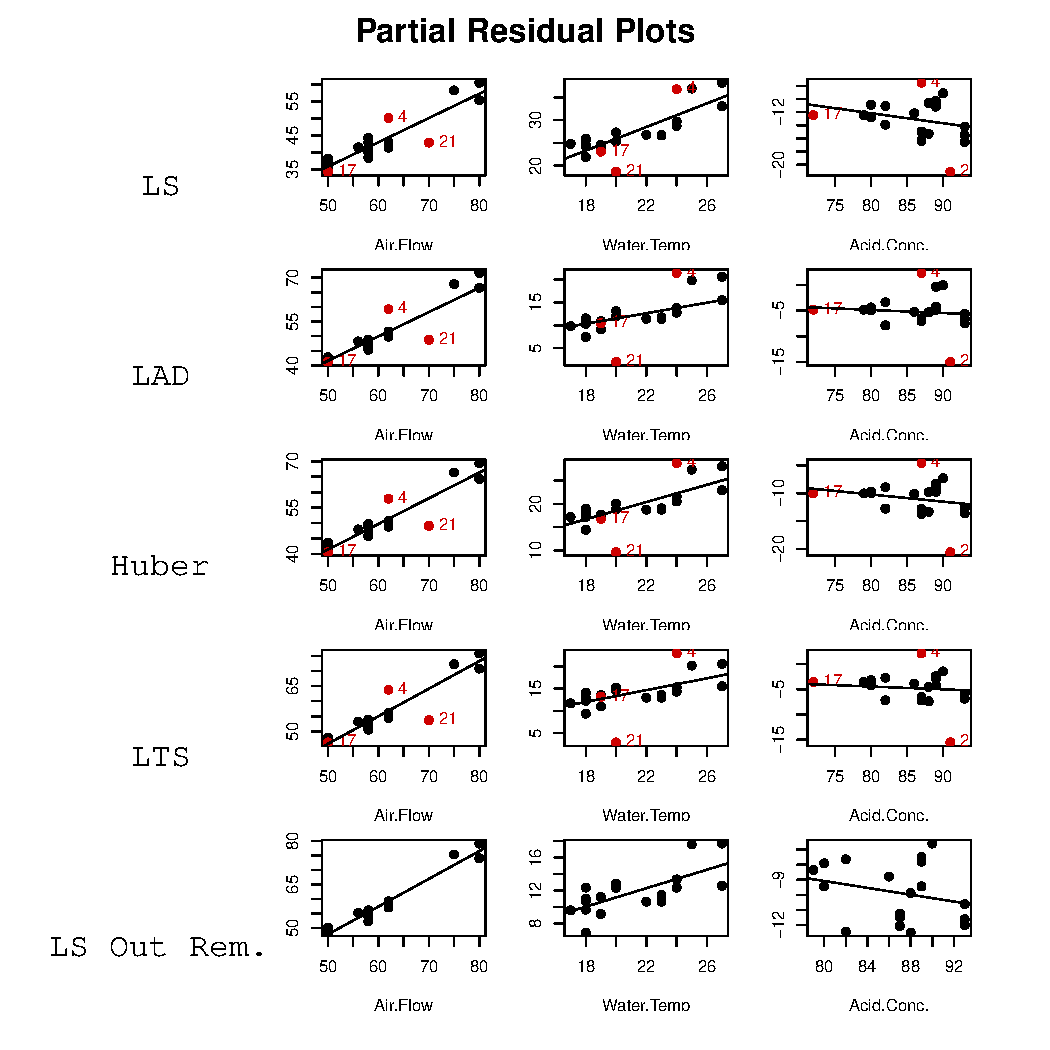
\includegraphics[width=\textwidth]{robust_matrix.pdf}
\end{minipage}
\begin{minipage}{.5\textwidth}
We first find those points that are influential or potential outliers as
outlined in homework 4.  Note that none of the adjusted residuals are
particularly extreme. Based on this table, we see that observations 4 and
21 are potentially troublesome. While observation 17 is influential, it seems to be well-predicted.
  So, for least-trimmed squares we will make our trimming quantile $n-2$.

We plotted a matrix of partial residual plots for each robust method.  The
points indicated in the table above are highlighted with larger red circles.

It appears that the least squares solution is influenced by observations 4 and 21
as they are outlying in water temperature.  Note, however, that they influence the
model in opposite directions.  
\end{minipage}
\begin{tabular}{c | l l l l l}
$\beta_i$  & LS & LAD & Huber & LTS & LS w/out 17,14,21\\\hline
(Intercept)& -39.920& -39.690& -41.027& -46.972& -42.059\\
Air.Flow   &   0.716&   0.832&   0.829&   0.917&   0.956\\
Water.Temp &   1.295&   0.574&   0.926&   0.667&   0.559\\
Acid.Conc. &  -0.152&  -0.061&  -0.128&  -0.056&  -0.114\\\hline
\end{tabular}

The estimates $\widehat \beta_i$ remain relatively unchanged except for water temperature.  Each robust estimate adjusts the water estimate estimate downward. Removing the outlying measurements most aggressively moves the estimate downward. 

Supposing we decide that LTS is best, we proceed in estimating the uncertainty in each $\widehat \beta_i$ by bootstrapping 5000 samples and reporting Bonferroni corrected 95\% confidence intervals based on the quantiles of the bootstrapped sample. We compare these with the intervals from the least squares estimates. Note that water temperature is significant in least squares but not in LTS and the model without 17,14, and 21.

\begin{verbatim}
Bootstrapped LTS
            estimate  0.625 % 99.375 %
(Intercept)  -46.972 -81.800 -13.940
Air.Flow       0.917   0.537   1.277
Water.Temp     0.667  -0.300   1.685
Acid.Conc.    -0.056  -0.490   0.376
\end{verbatim}

\begin{verbatim}
Least Squares
            estimate 0.625 %   99.375 %
(Intercept) -39.920  -73.140   -6.700
Air.Flow      0.716    0.339    1.092
Water.Temp    1.295    0.268    2.323
Acid.Conc.   -0.152   -0.589    0.284
\end{verbatim}

\begin{verbatim}
Least Squares w/out 17,14,21
            estimate  0.625   % 99.375 %
(Intercept) -42.059  -69.949  -14.170
Air.Flow      0.956    0.674    1.238
Water.Temp    0.559   -0.237    1.354
Acid.Conc.   -0.114   -0.468    0.241
\end{verbatim}

\end{solution}

\problem{ Faraway 14.3. Using the \texttt{PlantGrowth} data, determine whether there are any differences between the groups.  What is the nature of these differences?  Test for a difference between the average of the two treatments and the control. }
\begin{solution}
  \begin{minipage}{.4\textwidth}
  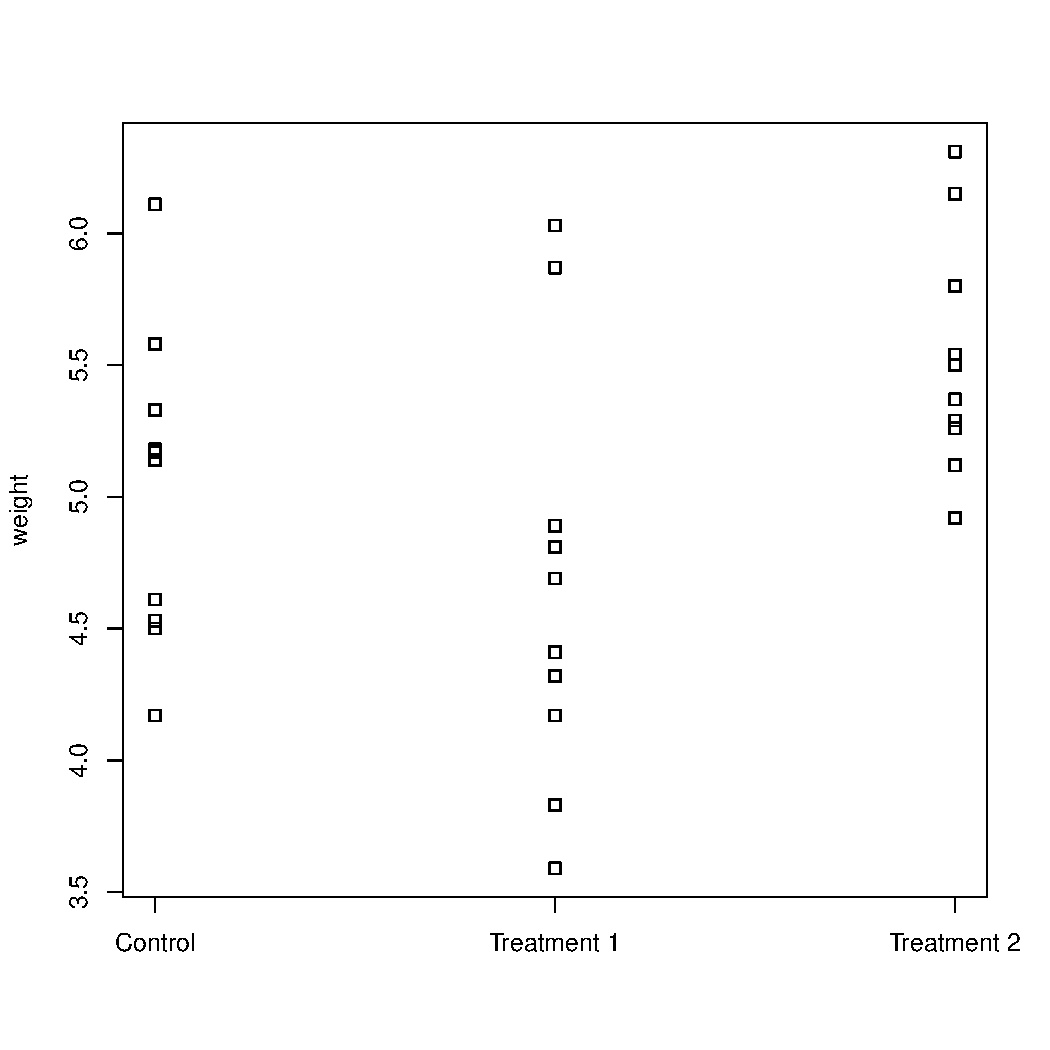
\includegraphics[width=\textwidth]{strip_plant.pdf}
  \end{minipage}
  \begin{minipage}{.55\textwidth}
  We fit an ANOVA model with one factor at three levels taking the control as the baseline. Note that the strip chart to the left does not indicate any reason to investigate non-homogeneous variance between levels.  The model fit is moderately significant at $F=4.846,p=0.016$.
  
  To test for an effect of the ``average treatment'', we test the significance of the contrast 
  $$H_0:\,l:= \mu_0 - \frac12(\mu_1 + \mu_2) = 0.$$  
The test yields $t=-0.255,p=0.400$, so there is absolutely no evidence of an effect.  Note that treatment 1 is lower than the control and treatment 2 is higher, and their individual effects are washed out by averaging.  
\end{minipage}
\end{solution}


\problem{ Read the paper titled ``Statistical Ritual vs.~Knowledge Accrual in
Wildlife Science'' by Fred Guthery, \emph{Journal of Wildlife Management},
72(8), pp. 1872-1874 (2008) and address the author's views on ``psuedodifferences'', AIC-based model selection, and the use of transformations in models in no more than one paragraph.}

\begin{solution}
In the article, the author argues that quantitative methods have largely supplanted ``knowledge
accrual'' and even common sense as the substance of research in wildlife science literature.  He
presents several abuses that fall into three categories -
abuse of significance testing by testing obvious and scientifically vacuous
hypotheses (significance testing) and detecting ``psuedodifferences'' by sampling with large $n$ effectively deflating standard errors; model selection that favors quantitative properties (e.g. AIC) over reasonable interpretability (quantitative debasement of research problems); and, similar to the last, overt embrace of quantitative techniques (such as esoteric transformations to satisfy variance homogeneity) that render reasonable interpretation impossible (results lacking information).  He does not offer much in the way of explaining why these practices have become prevalent other than anecdotally referring to human tendency toward ritual.
\end{solution}

\problem{ Write a paragraph summary of what you plan to do as your final project for this course. }

I plan on investigating methods for estimating variance in a random response in the pressence of measurement error when repeated measurements are taken.  We model the $n$ experiments with $m$ measurements as 
$$
  \vect y = \vect{X\beta} + \vect{P\eta} + \vect \epsilon
$$
where $\vect y$ is the response, $\vect{X\beta}$ are fixed linear predictors,
$\vect{P\eta}$ is the modeled random variation in the experiment, and $\vect
\epsilon$ is random measurement error.  In
particular, I plan on contrasting two methods, an iterative method and a REML
of a mixed effect model.  Pending authorization, these methods will be
presented on actual data.
\end{document} 

